

\chapter[Prediktivni modeli primjenom strojnog učenja]{Prediktivni modeli primjenom \\ strojnog učenja}

Kako bismo bolje razumjeli što film čini uspješnim ili neuspješnim, provele smo analizu dobivenog skupa podataka primjenom strojnog učenja. Cilj nam je bio razviti model koji može čim točnije predviđati uspjeh filma na temelju njegovih karakteristika.
\\
\section{Priprema podataka}
Iz dobivenih podataka izbacile smo retke kojima su nedostajali neki podaci. Takvih je redaka bilo 1261. Također, uklonile smo stupce koji su sadržavali jedinstvene ili skoro jedinstvene vrijednosti (\textit{movie\_title, movie\_imdb\_link, plot\_keywords, genres}). Još smo izbacile tekstualne stupce koji su bili prekorelirani s nekim numeričkim stupcem. Na primjer, \textit{actor\_1\_name} je prekoreliran s \textit{actor\_1\_facebook\_likes}. 

\lstinputlisting[language=R]{../R/001.R} 
Preostale nenumeričke stupce pretvorile smo u tip integer. 

\lstinputlisting[language=R]{../R/002.R}

Značajka koju predviđamo je \textit{imdb\_score}. To broj zaokružen na jednu decimalu, pa smo za bolje rezultate uspjeh filma podijelile u tri skupine: loš, osrednji i dobar, a stupac imdb\_score smo zbog prekoreliranosti uklonile. 

\lstinputlisting[language=R]{../R/003.R}

Graf \ref{fig:ml1} prikazuje omjer broja filmova po uspjehu. Filmova koji su ocijenjeni kao loši znatno je manje od ostalih. Točnije, loših je filmova 43, osrednjih 1981, a dobrih 1746.

\begin{figure}[H]
	\centering
	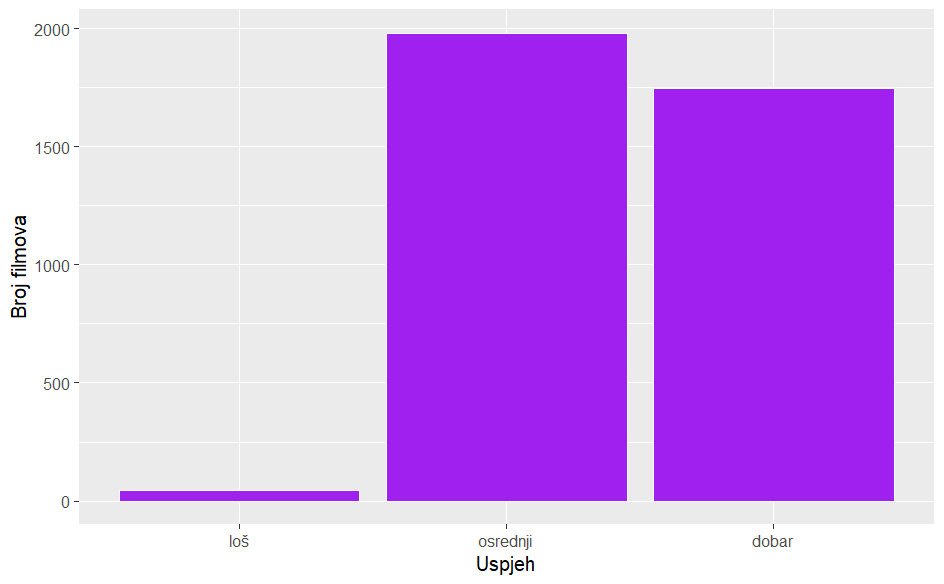
\includegraphics[width=15cm]{../figures/expl/001.png}
	\caption{Podjela filmova po uspjehu}
	\label{fig:ml1}
\end{figure}

\section{Modeli s nebalansiranim skupom podataka}
Kako bismo razvile model za predviđanje uspješnosti, skup podataka podijelile smo u omjeru 80:20. Na temelju 80\% gradile smo model, a na 20\% ga testirale. \\
Prvi model koji smo razvile koristi metodu potpornih vektora. 

\lstinputlisting[language=R]{../R/004.R}

Model radi s uspješnošću od 72.8\%.

\begin{figure}[H]
	\centering
	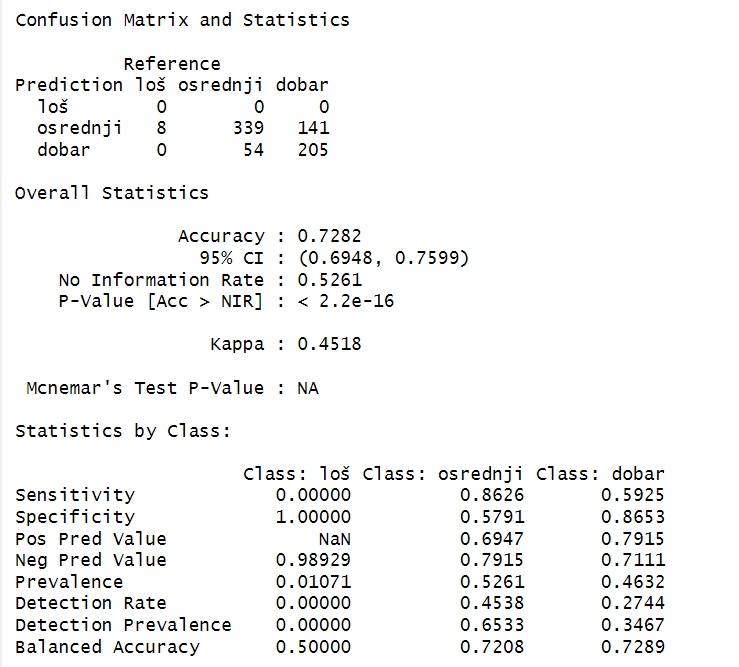
\includegraphics[width=15cm]{../figures/expl/002.png}
	\caption{Metoda potpornih vektora - rezultati}
	\label{fig:ml2}
\end{figure}

Drugi model koji smo razvile koristi metodu slučajne šume. Rezultati su nešto bolji, uspješnost je 78.3\%.

\lstinputlisting[language=R]{../R/005.R}

\begin{figure}[H]
	\centering
	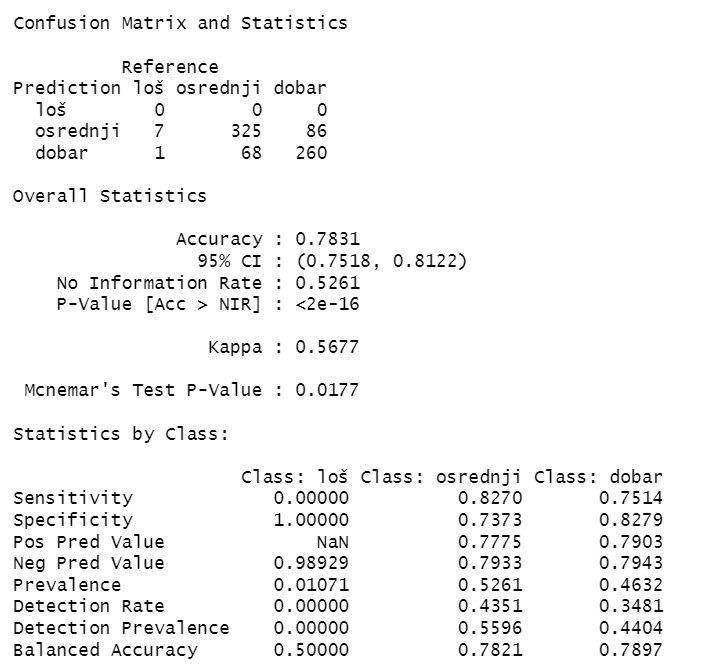
\includegraphics[width=15cm]{../figures/expl/003.png}
	\caption{Metoda slučajne šume - rezultati}
	\label{fig:ml3}
\end{figure}

Iako su ovi rezultati na prvi pogled donekle zadovoljavajući, nijedan od ovih modela nije predvidio da će ijedan film biti loš. To je očekivani rezultat jer podaci nisu nimalo balansirani - loših filmova je znatno manje pa ih je i puno teže predvidjeti. Produkciji filma bilo bi najkorisnije imati model koji može predvidjeti neuspjeh filma, a ovi modeli to ne uspijevaju pa smo ih odbacile.

\section{Modeli s balansiranim skupom podataka}

S ciljem poboljšanja točnosti predviđanja loših filmova, podatke smo balansirale. Nastojale smo broj loših i dobrih filmova približiti broju osrednjih filmova ( Graf \ref{fig:ml4} ).

\lstinputlisting[language=R]{../R/006.R}

\begin{figure}[H]
	\centering
	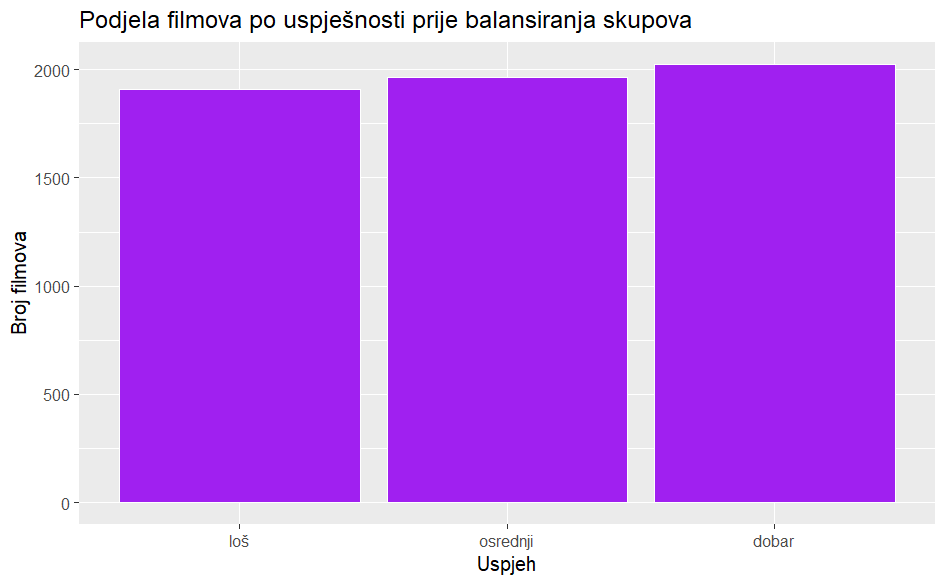
\includegraphics[width=15cm]{../figures/expl/004.png}
	\caption{Podjela filmova po uspjehu - balansirani podaci}
	\label{fig:ml4}
\end{figure}

Nad novim smo podacima ponovo testirale naše modele. Ovaj je put metoda potpornih vektora postigla uspješnost od 75.6\% ( Slika \ref{fig:ml5} ), a metoda slučajne šume visokih 90.9\%  ( Slika \ref{fig:ml6} ).

\begin{figure}[H]
	\centering
	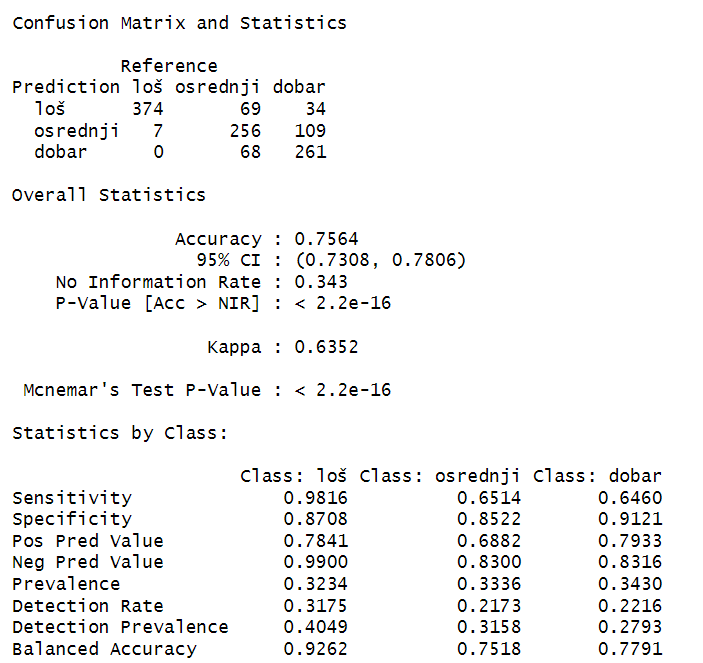
\includegraphics[width=15cm]{../figures/expl/005.png}
	\caption{Metoda potpornih vektora - rezultati s balansiranim podacima}
	\label{fig:ml5}
\end{figure}

\begin{figure}[H]
	\centering
	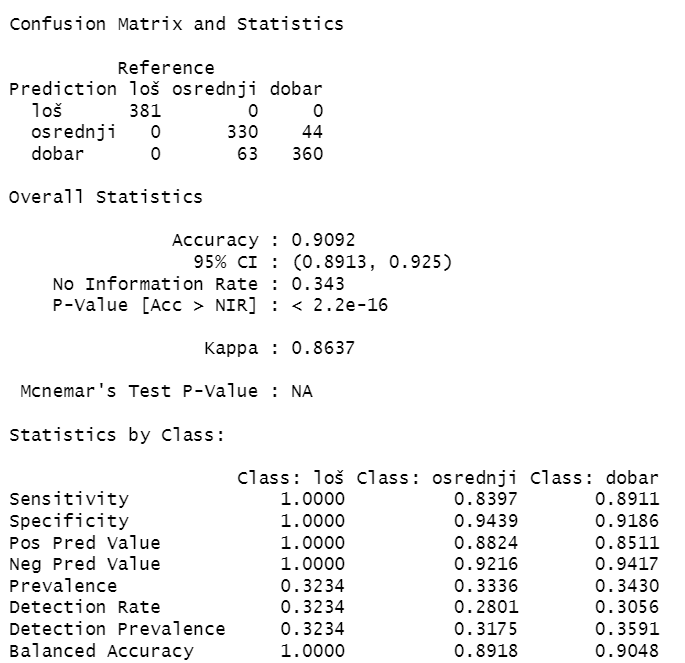
\includegraphics[width=15cm]{../figures/expl/006.png}
	\caption{Metoda slučajne šume - rezultati s balansiranim podacima}
	\label{fig:ml6}
\end{figure}

Ovim smo rezultatima zadovoljne jer oba modela s visokom točnošću predviđaju loše filmove.

\section{Atributi najznačajniji za predviđanje}

Idući je korak u analizi bio otkriti koji atributi najviše koriste pri predviđanju uspješnosti filmova, posebice onih loših.

Analizu smo provele nad modelom koji koristi metodu slučajne šume i balansirani skup podataka jer upravo taj model daje najbolje rezultate.

Atributi koji su u našem modelu u najvećoj korelaciji s uspješnosti su trajanje i broj negativnih recenzija. 

Filmovi koji su dobili loše ocjene gledatelja najčešće traju između sat i dva sata, a većina ih traje do 100 minuta. Grafovi za ostale filmove također prikazuju da najviše filmova traje 100 ili više minuta.

\begin{figure}[H]
	\centering
	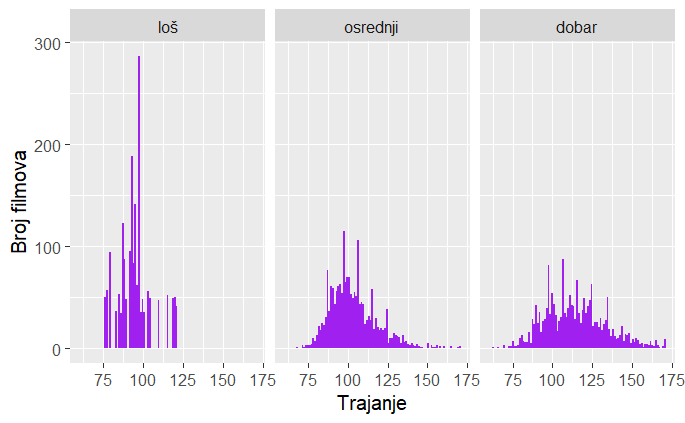
\includegraphics[width=15cm]{../figures/expl/007.png}
	\caption{Histogram trajanja filmova u ovisnosti o uspjehu}
	\label{fig:ml7}
\end{figure}

Za predviđanje uspješnih i neuspješnih filmova bio je važan i broj negativnih recenzija. Zanimljivo, filmovi koje smo klasificirale kao neuspješne imali su manji broj negativnih recenzija. Razlog tome je vjerojatno taj što se velik broj ljudi odlučio uopće ne pogledati film kad je vidio da je većina recenzija negativna. Uspješnije filmove pogleda puno više ljudi različitih mišljenja pa je očekivano da se nekima neće svidjeti. Ovaj trend potvrđuje i graf na slici \ref{napredni4}.

\begin{figure}[H]
	\centering
	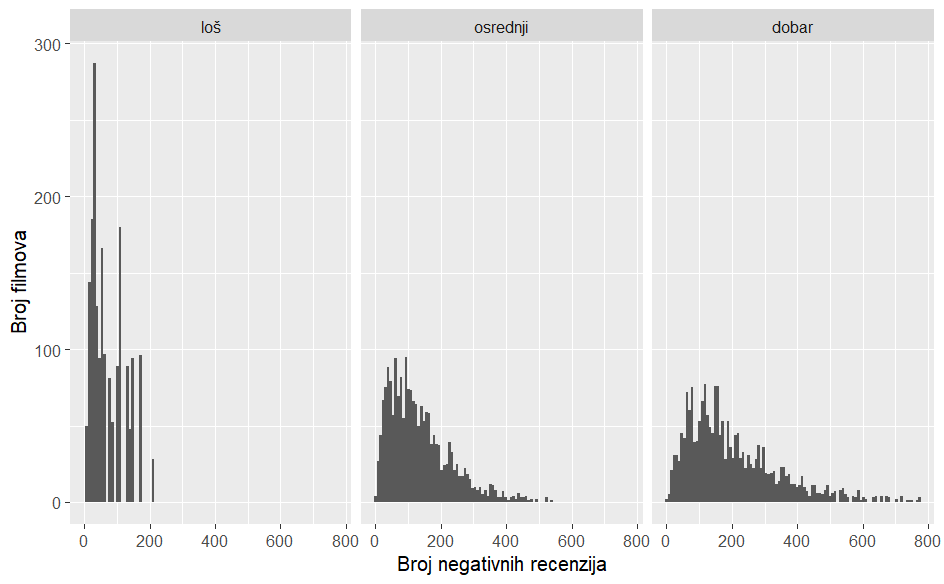
\includegraphics[width=15cm]{../figures/expl/008.png}
	\caption{Prikaz broja negativnih recenzija u ovisnosti o uspjehu}
	\label{fig:ml8}
\end{figure}

Atributi koji su najmanje korelirani s uspjehom filma su jezik i broj ljudi na plakatu.

\eject